\documentclass[a4paper,12pt, leqno]{article}
\usepackage{amsmath,amsthm,amssymb,enumitem, cclicenses, hyperref,amsfonts,tikz-cd,mathrsfs, tikz}
\usetikzlibrary{matrix, calc, arrows}
\setlength{\parindent}{0cm}
\setlength{\parskip}{6pt}
\tikzset{
	curvedlink/.style={
		to path={
			let \p1=(\tikztostart.east), \p2=(\tikztotarget.west),
			\n1= {abs(\y2-\y1)/4} in
			(\p1) arc(90:-90:\n1) -- ([yshift=2*\n1]\p2) arc (90:270:\n1)
		},
	}
}
\newcommand{\homo}{\mathrm{Hom}}
\newcommand{\Q}{\mathbb{Q}}
\newcommand{\Z}{\mathbb{Z}}
\newcommand{\im}{\mathrm{im}\,}
\newcommand{\id}{\mathrm{id}}
\newcommand{\ind}{\mathrm{Ind}_G}
\DeclareMathOperator{\coker}{coker}

\newtheoremstyle{defprop} % name
{\topsep}                    % Space above
{\topsep}                    % Space below
{\mdseries}                  % Body font
{}                           % Indent amount
{\bfseries}                   % Theorem head font
{.}                          % Punctuation after theorem head
{.5em}                       % Space after theorem head
{}  % Theorem head spec (can be left empty, meaning ‘normal’)
 
\newtheoremstyle{dem} % name
{\topsep}                    % Space above
{\topsep}                    % Space below
{\mdseries}                  % Body font
{}                           % Indent amount
{\itshape}                   % Theorem head font
{.}                          % Punctuation after theorem head
{.5em}                       % Space after theorem head
{}  % Theorem head spec (can be left empty, meaning ‘normal’)          

\newtheoremstyle{prop} % name
{\topsep}                    % Space above
{\topsep}                    % Space below
{\itshape}                  % Body font
{}                           % Indent amount
{\bfseries}                   % Theorem head font
{.}                          % Punctuation after theorem head
{.5em}                       % Space after theorem head
{}  % Theorem head spec (can be left empty, meaning ‘normal’)   

\newtheoremstyle{teor} % name
{\topsep}                    % Space above
{\topsep}                    % Space below
{\itshape}                  % Body font
{}                           % Indent amount
{\bfseries}                   % Theorem head font
{.}                          % Punctuation after theorem head
{.5em}                       % Space after theorem head
{}  % Theorem head spec (can be left empty, meaning ‘normal’)               

\theoremstyle{defprop}
\newtheorem{defprop}{Definición/Proposición}
\newtheorem{definicion}{Definición}
\newtheorem*{ejemplo}{Ejemplo}

\theoremstyle{prop}
\newtheorem{prop}{Proposición}

\theoremstyle{teor}
\newtheorem{teor}{Teorema}

\theoremstyle{dem}
\newtheorem*{dem}{Demostración}

%Flechas
\newcommand\rightthreearrow{%
	\mathrel{\vcenter{\mathsurround0pt
			\ialign{##\crcr
				\noalign{\nointerlineskip}$\rightarrow$\crcr
				\noalign{\nointerlineskip}$\rightarrow$\crcr
				\noalign{\nointerlineskip}$\rightarrow$\crcr
			}%
	}}%
}

\newcommand\rightfourarrow{%
	\mathrel{\vcenter{\mathsurround0pt
			\ialign{##\crcr
				\noalign{\nointerlineskip}$\rightarrow$\crcr
				\noalign{\nointerlineskip}$\rightarrow$\crcr
				\noalign{\nointerlineskip}$\rightarrow$\crcr
				\noalign{\nointerlineskip}$\rightarrow$\crcr
			}%
	}}%
}



\title{Día 2}
\author{Daniel M.}

\begin{document}
\maketitle
Salvo que se indique todo lo contrario $G$ será un grupo profinito y todos los $G$-módulos vendrán equipados con la topología discreta. 
\begin{definicion} 
	Sea $(I,\leq)$ un conjunto parcialmente ordenado y dirigido. Sea $\{A_i\}_{i \in I}$ una familia de objetos en una categoría $\mathcal{A}$ y sea $\{f_{ij}\}_{i\leq j}$ una familia de morfismos que verifican $f_{ij}\in \mathrm{Mor}(A_i,A_j)$, $f_{ii}=\id_{A_i}$ y $f_{ik}=f_{jk}\circ f_{ij}$ para $i\leq j \leq k$. Al par $((A_i)_{i \in I}, (f_{ij})_{i\leq j})$ le llamamos un \textbf{sistema directo}.
	
	Un \textbf{límite directo} es un par $(X,(\phi_i)_{i\in I})$ donde $X$ es un objeto en la categoría, $\phi_i: X_i \rightarrow X$ verifican $\phi_i = \phi_j \circ f_{ij}$ para $i \leq j$ y además para cualquier otro $(Y,(\psi_i)_{i\in I})$ con la misma propiedad hay un único morfismo $u:X \rightarrow Y$ tal que el siguiente diagrama conmuta: 

	\begin{center}
			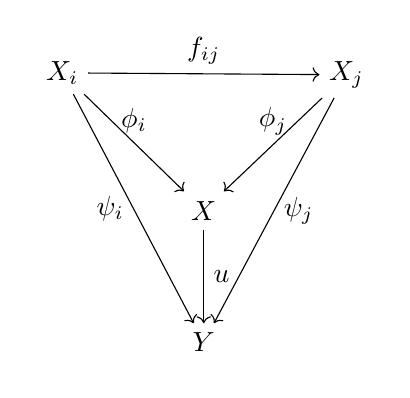
\begin{tikzpicture}
		\centering
			\matrix[matrix of nodes,ampersand replacement=\&, column sep=1.2cm, row sep=1.2cm](m)
		{
			$X_i$ \& \& $X_j$ \\
			\& $X$ \&  \\
			\& $Y$ \&  \\		
		};
		
		\draw[->] (m-1-1) edge node[above] {$f_{ij}$} (m-1-3)
		(m-1-1) edge node[above] {$\phi_i$}(m-2-2) 
		(m-1-3) edge node[above] {$\phi_j$}  (m-2-2)
		(m-1-1)  edge node[left] {$\psi_i$}(m-3-2) 
		(m-1-3) edge node[right] {$\psi_j$} (m-3-2)
		(m-2-2) edge node[midway,right] {$u$} (m-3-2)
		;
		\end{tikzpicture}
	\end{center}
A una propiedad de ese tipo se le denomina una \textit{propiedad universal}. La notación para el límite directo es $X=\varinjlim A_i$.
\end{definicion}
\begin{prop}
	El límite directo es único salvo isomorfismo. 
\end{prop}
\begin{dem}
	
	
	Con la misma notación que antes, sean $(X,(\phi_i)_{i\in I})$ y $(Y,(\psi_i)_{i\in I})$ dos límites inversos. Por la propiedad universal, sabemos que existen dos morfismos únicos $u:X \rightarrow Y$ y $v:Y \rightarrow X$ tal que $\phi_i=v \circ \psi_i$ y $\psi_i = u \circ \phi_i$.
	
	Combinando ambas obtenemos $\phi_i=v \circ u \circ \phi_i$ y también $\psi_i = u \circ v \circ \psi_i$. Como $u,v$ son únicas y $\id_X,\id_Y$ satisfacen las identidades, deducimos que $u\circ v=\id_X$ y $v \circ U = \id_Y$ de lo que deducimos que son isomorfismos.\qed
\end{dem}	
\begin{prop}
La categoría de $R$-módulos tiene límites directos	
\end{prop}

A continuación podemos estudiar cómo los grupos de cohomología $H^n(G,A)$ de un grupo profinito $G$ con coeficientes en $A$ se construyen a partir la cohomología de cocientes los $G/U$, donde $U$ es un subgrupo normal y abierto.  

Dados dos subgrupos normales y abiertos $V\subseteq U$ de $G$, las proyecciones canónicas:
\begin{equation*}
G^{n+1}\rightarrow (G/V)^{n+1} \rightarrow (G/U)^{n+1}
\end{equation*}
inducen homomorfismos de complejos de cocadenas:
\begin{equation*}
C^{\bullet}(G/U,A^U) \rightarrow C^{\bullet}(G/V,A^V) \rightarrow C^{\bullet}(G,A).
\end{equation*}
De aquí obtenemos homomorfismos:
\begin{equation*}
H^n(G/U,A^U) \rightarrow H^n(G/V,A^V)\rightarrow H^n(G,A).
\end{equation*}
Es decir, los grupos $H^n(G/U,A^U)$ donde $U$ recorre subgrupos normales y abiertos forman un sistema directo con un homomorfismo canónico:
\begin{equation*}
\varinjlim\limits_{U} H^n(G/U,A^U) \rightarrow H^n(G,A).
\end{equation*}
\begin{prop}\label{prop3}
El homomorfismo canónico es en realidad un isomorfismo:
\begin{center}
	\begin{tikzcd}
	\varinjlim\limits_{U} H^n(G/U,A^U)\arrow{r}{\sim} & H^n(G,A).
	\end{tikzcd}
\end{center}
\end{prop}
\begin{dem}
El homomorfismo de complejos:
\begin{equation*}
\varinjlim\limits_{U} C^{\bullet}(G/U,A^U) \rightarrow C^{\bullet}(G,A)
\end{equation*}
es en realidad un isomorfismo. La inyectividad se sigue de la inyectividad de los homomorfismos $C^{\bullet}(G/U,A^U)\rightarrow C^{\bullet}(G,A)$. 

Para ver que es sobreyectivo, sea $x:G^{n+1}\rightarrow A$ una cocadena de $G$.  Como $A$ tiene la topología discreta $x$ es localmente constante. Afirmo que podemos encontrar un subgrupo normal y abierto $H_0$ de $G$ tal que $x$ es constante en las clases laterales de $H_0^{n+1}$ en $G^{n+1}$.

Por compacidad, sea $\im x = \{a_1,...,a_n\}$ y sean $U_i=x^{-1}(a_i)$. Como los $U_i$ son abiertos, los podemos escribir como una unión de clases laterales $U_i = \cup g_i H_i$, donde los $H_i$ son abiertos y normales. Como además $U_i$ es cerrado y por tanto compacto, la unión es finita y de la forma $g_i H$ si tomamos $H$ la interseccion de los correspondientes $H_i$. Tomando un $H_0$ suficientemente pequeño logramos escribir todos los $x^{-1}(a_i)$ como una unión de clases laterales de $H_0$ y obtenemos que $x$ es constante en ellas. Todo esto lo podemos hacer por que al ser $G$ profinito hay una base fundamental de entornos del elemento neutro formada por subgrupos abiertos. Además tenemos que para $h \in H_0$:
\begin{equation*}
x(\sigma_0,...,\sigma_n)=x(h \sigma_0,...,h \sigma_n)=h x(\sigma_0,...,\sigma_n),
\end{equation*}
luego $x$ factoriza de la siguiente manera:
\begin{center}
	\begin{tikzcd}
	G^{n+1}\arrow{r} &(G/H_0)^{n+1} \arrow{r}{x_{H_0}} & A^{H_0},
	\end{tikzcd}
\end{center}
y $x$ es la imagen de la clase de $x_{H_0}$ en $\varinjlim\limits_{U} C^n(G/U,A^U)$. Luego efectivamente es sobreyectivo. Para terminar utilizamos que $\varinjlim$ es un un functor exacto:
\begin{align*}
\varinjlim\limits_{U} H^n(G/U,A^U)& \simeq H^n\varinjlim\limits_{U} C^{\bullet}(G/U,A^U)\\
&\simeq H^n(C^{\bullet}(G,A))\\
&= H^n(G,A).
\end{align*}\qed

\end{dem}
\section{Cohomología de Tate para grupos finitos}
Sea $G$ un grupo finito en esta sección. Denotamos por $N_G: A \rightarrow A$ la función norma $N_G a = \sum_{g \in G}ga$ y sean:
  \[
\hat{H}^n(G,A) =\left\{ \begin{array}{lr}
A^G/N_GA, & \text{para } n= 0\\
H^n(G,A) & \text{para } n\geq 1,
\end{array}\right.
\]
a los que denominamos \textbf{grupos modificados de cohomología}. Además de $A^G$ podemos definir un módulo de elementos cofijos $A_G=A / I_GA$, donde $I_GA$ es el subgrupo de $A$ generado por elementos de la forma $ga-a,a\in A$ y $g\in G$. $A_G$ es el cociente más grande de $A$ en el que $G$ actúa trivialmente. Sea $H_0(G,A)=A_G$.

Nótese que siempre que $G$ sea finito, $I_GA\subseteq \ker N_G = {}_{N_G}A$, luego podemos denotar:
\begin{equation*}
\hat{H}_0(G,A)={}_{N_G}A/I_GA.
\end{equation*}
Todo esto nos da una sucesión exacta:
\begin{center}
	\begin{tikzcd}
	0 \arrow{r} & \hat{H}_0(G,A) \arrow{r}& H_0(G,A) \arrow{r}{N_G} & H^0(G,A) \arrow{r} & \hat{H}^0(G,A) \arrow{r} & 0,
	\end{tikzcd}
\end{center}
donde $N_G:H_0(G,A)\rightarrow H^0(G,A)$ es inducida por $N_G$. El primer y el último término que no son cero son respectivamente el núcleo y conúcleo de $N_G$.

A continuación vamos a extender nuestros grupos de cohomología a todo $n \in \mathbb{Z}$. Para $n\geq 0$, sea $\mathbb{Z}[G^{n+1}]$ el grupo abeliano libre generado por elementos de $G^{n+1}$, que tiene estructura de $G$-módulo. Consideremos la \textbf{resolución estándar completa} de $\Z$:
\begin{center}
	\begin{tikzcd}
	\cdot \arrow{r}& X_2 \arrow{r}{\partial_2}& X_1 \arrow{r}{\partial_1}& X_0 \arrow{r}{\partial_0}& X_{-1} \arrow{r}{\partial_{-1}}&X_{-2} \arrow{r} & \cdots
	\end{tikzcd}
\end{center}
donde $X_n=X_{-1-n}=\Z[G^{n+1}]$ para $n\geq 0$ y los homomorfismos para $n>0$ son:
\begin{align*}
\partial_n(\sigma_0,...,\sigma_n)&=\sum_{i=0}^{n}(-1)^i(\sigma_0,...,\sigma_{i-1},\sigma_{i+1},...,\sigma_n)\\
\partial_{-n}(\sigma_0,...,\sigma_{n-1})&=\sum_{\tau \in G}\sum_{i=0}^{n}(-1)^i(\sigma_0,...,\sigma_{i-1},\tau,\sigma_{i+1},...,\sigma_{n+1}).
\end{align*}
A su vez definimos $\partial_0: X_0 \rightarrow X_{-1}$ como:
\begin{equation*}
\partial_0(\sigma_0)=\sum_{\tau \in G}\tau.
\end{equation*}
A partir de esto, la \textbf{resolución estándar completa} de A se define tomando $X^{\bullet}(X_{\bullet},A),\partial^n= \homo (\partial_n,A)$ para $n \in \Z$.  Uno puede demostrar que el complejo $X^{\bullet}$ es exacto porque la identidad es null-homotópica.

\begin{definicion}
	Para $n\in \Z$ definimos el enésimo grupo de cohomología de Tate $\hat{H}(G,A)$ como el grupo de cohomología del complejo:
	\begin{equation*}
	\hat{C}^{\bullet}(G,A)=((X^n)^G)_{n \in \Z}
	\end{equation*}
	en el término $n$:
	\begin{equation*}
	\hat{H}^n(G,A)=H^n(	\hat{C}^{\bullet}(G,A)).
	\end{equation*}
\end{definicion}
Obsérvese que para $n\geq 0 $ obtenemos los grupos d e cohomología modificados de antes y que para $n=-1$ obtenemos $\hat{H}_0(G,A)$. Las dimensiones negativas corresponden a la homología, algo que veremos más adelante. 
\section{Módulos inducidos}
Dada una sucesión exacta corta:
\begin{equation*}
0 \rightarrow A \rightarrow B \rightarrow C \rightarrow 0
\end{equation*}
con su correspondiente sucesión larga, es importante observar que si se verifica $H^n(G,B)=H^{n+1}(G,B)=0$ para algún $n$ entonces:
\begin{equation*}
\delta: H^n(G,C)\rightarrow H^{n+1}(G,A)
\end{equation*}
es un isomorfismo, lo cual motiva la siguiente definición:
\begin{definicion}
	Un $G$-módulo $A$ es \textbf{acíclico} si $H^n(G,A)=0$ para todo $n>0$. $A$ es \textbf{cohomológicamente trivial} si $H^n(H,A)=0$ para todos los subgrupos cerrados $H\leq G$ y para todo $n>0$.
\end{definicion}
Un ejemplo importante de módulos cohomológicamente triviales son los $G$-módulos inducidos:
\begin{equation*}
\ind(A)=\mathrm{Map}(G,A),
\end{equation*}
es decir las funciones continuas $x: G \rightarrow A$ con la acción dada por $(\sigma x)(g)=\sigma x(\sigma^{-1} g)$. Cuando $G$ es finito tenemos un isomorfismo:
\begin{equation*}
\ind (A) \cong A \otimes \Z[G]
\end{equation*}
dado por $x \mapsto \sum_{g \in G}x(g) \otimes g$.
\begin{prop}
	\begin{enumerate}[label=\roman*)]
		\item El functor $A \mapsto \ind (A)$ es exacto. 
		\item Un $G$-módulo inducido $A$ también es un $H$-módulo inducido para todo subgrupo cerrado $H\leq G$. Además si $H$ es normal, $A^H$ es un $G/H$-módulo inducido.
		\item $A \otimes B$ es $G$-inducido si uno de los dos lo es. Lo mismo es cierto para $\homo(A,B)$ si $G$ es finito. 
		\item Si $U$ recorre los subgrupos normales abiertos de $G$, tenemos:
		\begin{equation*} 
		\ind (A)= \varinjlim\limits_U \mathrm{Ind}_{G/U}(A^U).
		\end{equation*}
	\end{enumerate}
\end{prop}
Como comentábamos, el resultado más importante de esta sección sobre módulos inducidos es el siguiente:
\begin{prop}
	Los $G$-módulos inducidos $M=\ind (A)$ son cohomológicamente triviales. Si además $G$ es finito, tenemos que $\hat{H}^n(G,M)=0$ para todo $n \in \Z$.
\end{prop}
\begin{dem}
	Consideramos las resoluciones estándar $X^{\bullet}(G,A)$ y $X^{\bullet}(G,\ind (A))$, es decir aquellas en las que:
	\begin{equation*}
	X^n=\mathrm{Map}(G^{n+1},A);X^n=\mathrm{Map}(G^{n+1},\ind (A))
	\end{equation*}
	 respectivamente. Tenemos una aplicación:
	 \begin{equation*}
	 X^n(G,\ind (A))^G \rightarrow X^n(G,A)
	 \end{equation*}
	 dada por $x(\sigma_0,...,\sigma_n)\mapsto y(\sigma_0,...,\sigma_n)=x(\sigma_0,...,\sigma_n)(1)$. De hecho, esto un isomorfismo (ejercicio: encontrar el inverso) luego tenemos un isomorfismo de complejos:
	 \begin{equation*}
	 C^{\bullet}(G,\ind (A))\cong X^{\bullet}(G,A).
	 \end{equation*}
	 El primer día demostramos que $X^{\bullet}(G,A)$ era exacta, luego:
	 \begin{equation*}
	 H^n(G,\ind (A))=H^n(C^{\bullet}(G,\ind (A)))=0
	 \end{equation*}
	 para $n\geq 1$. Si $H$ es  un subgrupo cerrado de $G$, por la proposición anterior podemos escribir $\ind (A)=\mathrm{Ind}_H(B)$ para algún $B$ y entonces: 
	 \begin{equation*}
	 H^n(H,\ind (A))=0.
	 \end{equation*}
	 
	 Cuando $G$ es finito, se puede repetir el argumento en el complejo extendido $(X^n)_{n \in \Z}$ para obtener $\hat{H}^n(G, \ind (A))=0$ para todo $n \in \Z$. \qed
\end{dem}
Este resultado nos permite aplicar una técnica conocida como \textit{dimension shifting} que consiste en reducir demostraciones sobre todos los grupos de cohomología a una única dimension. Dado $A$, definimos $A_1$ con la siguiente sucesión exacta:
\begin{center}
	\begin{tikzcd}
	0 \arrow{r}& A \arrow{r}{i} & \ind (A) \arrow{r} & A_1 \arrow{r} & 0,
	\end{tikzcd}
\end{center}
donde $ia$ es la función constante $ia(\sigma)=a$. Si $H\leq G$ es un subgrupo cerrado, por la proposición anterior tenemos que el homomorfismo:
\begin{equation*}
\delta: H^n(H,A_1) \rightarrow H^{n+1}(H,A)
\end{equation*} 
es sobreyectivo para $n=0$ y un isomorfismo para $n>0$. Aplicando el mismo proceso inductivamente para $A_0 = A$ y $A_+=(A_{p-1})_1$ para $p>0$ obtenemos:
\begin{prop}\label{dimsh}
	Para $n,p \geq0$ y cualquier subgrupo $H$ de $G$, tenemos un homomorfismo canónico:\begin{equation*}
	\delta^p: H^n(H,A_p) \rightarrow H^{n+p}(H,A)
	\end{equation*}
	que es sobreyectivo para $n=0$ y un isomorfismo para $n>0$.
\end{prop}

Si $G$ es un grupo finito, también podemos obtener un resultado parecido para la cohomología de Tate. Consideremos la sucesión exacta:
\begin{center}
	\begin{tikzcd}
	0 \arrow{r}& A_{-1} \arrow{r}& \ind (A) \arrow{r}{\nu} & A \arrow{r} &0,
	\end{tikzcd}
\end{center}
donde $\nu:x \mapsto \sum_{g \in G} x(g)$. Definimos $A_p=(A_{p+1})_{-1}$ para $p<0$; utilizando que $\ind (A) \cong A \otimes \Z[G]$ es fácil ver que:
\begin{center}
	$A_p \cong A \otimes J_G^{\otimes p}$ y $A_{-p}\cong I_G^{\otimes p}$
\end{center}
para $p\geq 0$, donde $I_G,J_G$ vienen dados por las sucesiones:
\begin{center}
	\begin{tikzcd}
	0 \arrow{r} & I_G \arrow{r} & \Z[G] \arrow{r}{\epsilon} & \Z \arrow{r}& 0,\\
		0 \arrow{r}& \Z \arrow{r}{N_G}&\Z[G] \arrow{r} & J_G \arrow{r} & 0.
		\end{tikzcd}
	\end{center}
A $\epsilon$ se le denomina \textit{augmentation map}:
\begin{equation*}
\epsilon: \sum_{\sigma \in G} a_{\sigma} \sigma \mapsto \sum_{\sigma \in G} a_{\sigma},
\end{equation*}
y al $G$-módulo $I_G$ se le llama \textit{augmentation ideal}. Como $\hat{H}^n(H,\ind (A))=0$, obtenemos isomorfismos canónicos:
\begin{equation*}
\hat{H}^n(H,A)\cong \hat{H}^{n-p}(H,A_p)
\end{equation*}
para todo $n,p \in \Z$.

Volviendo a caso general de un grupo profinito $G$, otra forma de calcular los grupos de cohomología es utilizando resoluciones acíclicas $Y^{\bullet}$ de $A$, en cuyo caso $H^n(G,A)\cong H^n(H^0(G,Y^{\bullet}))$ (ver Proposición 1.3.9).
\section{El producto cup}
Recordamos que dados dos $G$-módulos $A$ y $B$, $A \otimes_{\mathbb{Z}} B$ con la acción diagonal también es un $G$-módulo. Esto nos permite definir para $p,q \geq 0 $:
\begin{center}
	\begin{tikzcd}
C^p(G,A)\times C^q(G,B) \arrow{r}{\cup}&  C^{p+q}(G, A \otimes B)
\end{tikzcd}
\end{center}
dado por:
\begin{equation*}
(a\cup b)(\sigma_0,...,\sigma_{p+q})=a(\sigma_0,...,\sigma_q)\otimes b(\sigma_p,...,\sigma_{p+q}).
\end{equation*}
Esta función verifica la siguiente formula:
\begin{equation*}
\partial(a \cup b)=(\partial a) \cup b + (-1)^p (a\cup \partial b),
\end{equation*}
que puede verificarse con un simple cálculo. Claramente, si $a$ y $b$ son cociclos entonces $a \cup b$ también es un cociclo. Además, si uno es  un cociclo y el otro es un coborde, $a \cup b$ también es un coborde. En definitiva, $\cup$ induce una aplicación bilineal:
\begin{center}
\begin{tikzcd}
H^p(G,A)\times H^q(G,B) \arrow{r}{\cup}&  H^{p+q}(G, A \otimes B),
\end{tikzcd}
\end{center}
dado por $(\alpha, \beta) \mapsto \alpha \cup \beta$. A esta aplicación le llamamos \textbf{producto cup}. También se le llama producto cup a la composición:
\begin{center}
	\begin{tikzcd}
	H^p(G,A) \times H^q(G,B) \arrow{r}{\cup} & H^{p+q}(G, A \otimes B)  \arrow{r} & H^{p+q}(G,C),
	\end{tikzcd}
\end{center}
que viene inducida por una aplicación bilineal $A \times B \rightarrow C$ que factoriza en el producto tensorial. 

Cada vez que definimos una aplicación nueva en la cohomología, tenemos que verificar sus propiedades functoriales y su compatibilidad con las anteriores. Directamente de la definición se sigue que el producto cup conmuta con homomorfismos $A \rightarrow A', B \rightarrow B'$. A continuación demostramos la compatibilidad con $\delta$:
\begin{prop}
	Sean
		
		\begin{center}
			 $0 \rightarrow A' \rightarrow A \rightarrow A'' \rightarrow 0$ y $0 \rightarrow C' \rightarrow C \rightarrow C''\rightarrow 0$.
		\end{center}
dos sucesiones exactas de $G$-módulos. Sea $B$ otro $G$-módulo y supongamos que existe un emparejamiento $A \times B \rightarrow C$ que induce $A' \times B\rightarrow C'$ y $A'' \times B \rightarrow C''$.  Entonces el diagrama siguiente conmuta:

\begin{center}
	\begin{tikzcd}[column sep=small]
	H^p(G,A'') \arrow[d,"\delta"] \arrow[r,phantom,"\times"] & H^q(G,B) \arrow[d,"id"] \arrow[r,"\cup"]& H^{p+q}(G,C'') \arrow[d,"\delta"]\\
	H^{p+1}(G,A') \arrow[r,phantom,"\times"]& H^q(G,B)  \arrow[r,"\cup"]&  H^{p+q+1}(G,C')
	\end{tikzcd}
\end{center}
Es decir, $\delta(\alpha'' \cup \beta)=\delta \alpha'' \cup \beta$.

Análogamente, dadas dos sucesiones exactas:
\begin{center}
	$0 \rightarrow B' \rightarrow B \rightarrow B'' \rightarrow 0$ y $0 \rightarrow C' \rightarrow C \rightarrow C''\rightarrow 0$
\end{center}
con un emparejamiento $A \times B \rightarrow C$ que induce $A \times B' \rightarrow C'$ y $A \times B'' \rightarrow C''$, el diagrama siguiente conmuta:
\begin{center}
	\begin{tikzcd}[column sep=small]
	H^p(G,A) \arrow[d,"id"] \arrow[r,phantom,"\times"] & H^q(G,B'') \arrow[d,"\delta"] \arrow[r,"\cup"]& H^{p+q}(G,C'') \arrow[d,"(-1)^p\delta"]\\
	H^{p}(G,A) \arrow[r,phantom,"\times"]& H^{q+1}(G,B')  \arrow[r,"\cup"]&  H^{p+q+1}(G,C').
	\end{tikzcd}
\end{center}
Es decir, $(-1)^p \delta(\alpha \cup \beta'') = \alpha \cup \delta \beta''$.
\end{prop}
\begin{dem}
	Demostramos la primera igualdad, siendo análoga la demostración de la segunda. Sean $\alpha''=\overline{a''},\beta=\overline{b}$ para $a''\in Z^p(G,A''),b\in Z^q(G,A)$. 
	
	El functor $A \mapsto C^p(G,A)$ es exacto, luego podemos elegir $a\in C^p(G,A)$ que esté en la preimagen de $a''$.	Entonces por definición de $\delta$, $\delta \alpha''\in H^{p+1}(G,A')$ es representado por $\partial a\in Z^{p+1}(G,A')$  (identificando $A'$ con su imagen en $A$).
	
	A su vez, $\delta(\alpha'' \cup \beta)$ es representado por $\partial(a \cup b)=\partial a \cup b$, ya que $\partial b = 0$. Pasando a cohomología esto significa:
	\begin{equation*}
	\delta(\alpha'' \cup \beta)=\delta \alpha'' \cup \beta.
	\end{equation*}\qed
\end{dem}
\begin{prop}
	El producto cup verifica:
	
	\begin{enumerate}[label = \roman*)]
		\item $(\alpha \cup \beta) \cup \gamma = \alpha \cup (\beta \cup \gamma)$.
		\item $\alpha \cup \beta = (-1)^{pq}(\beta \cup \alpha)$.
	\end{enumerate}
\end{prop}
\begin{dem}
	La primera afirmación es una comprobación directa. Para la segunda utilizaremos el método de \textit{dimension shifting} introducido en la Proposición \ref{dimsh}. Recordamos que existen homomorfismos sobreyectivos $\delta^n: H^0(G,A_n)\rightarrow H^n(G,A).$ Aplicando la proposición anterior $p$ y $q$ veces respectivamente obtenemos un diagrama conmutativo:
	\begin{center}
		\begin{tikzcd}
		[column sep=small]
		H^0(G,A_p) \arrow[d,"\delta^p"] \arrow[r,phantom,"\times"] & H^0(G,B_q) \arrow[d,"id"] \arrow[r,"\cup"]& H^0(G,(A\otimes B_q)_p) \arrow[d,"\delta^p"] \arrow[r,phantom,"="]& H^0(G,A_p \otimes B_q)\\
		H^p(G,A') \arrow[r,phantom,"\times"] \arrow[d,"id"]& H^0(G,B_q)  \arrow[r,"\cup"] \arrow[d,"\delta^p"]&  H^p(G,(A \otimes B)_q) \arrow[d,"(-1)^{pq}\delta^q"] \arrow[r,phantom,"="] & H^p(G,A \otimes B_q)\\
		H^p(G,A\arrow[r,phantom,"\times"] & H^q(G,B) \arrow[r,"\cup"] & H^{p+q}(G,A\otimes B)
		\end{tikzcd}	
\end{center}
Para $p=q=0$ la identidad es trivial. Como las flechas verticales son sobreyectivas, obtenemos $\alpha \cup B=(-1)^{pq}(\beta \cup \alpha)$ para $p,q \geq 0$.\qed
\end{dem}
%\begin{prop}
%	Sean:
%	\begin{center}
%		$0 \rightarrow A' \rightarrow A \rightarrow A'' \rightarrow 0$ y $0 \rightarrow B' \rightarrow B \rightarrow B'' \rightarrow 0$
%	\end{center}
%dos sucesiones exactas de $G$-módulos tal que existe un emparejamiento $\phi: A \times B \rightarrow C$ con $C$ otro $G$-módulo y tal que $\phi(A' %\times B')=0$. Es decir, $\phi$ induce $\phi',\phi''$ tal que el siguiente diagrama conmuta:
%\begin{center}
%	\begin{tikzcd}
%	A' \arrow[r,phantom,"\times"] \arrow[d,hook,"i"] & B'' \arrow[r,"\phi'"] & C \arrow[d,equal]\\
%	A \arrow[d,two heads,"j"] \arrow[r,phantom,"\times"] & B \arrow[u, two heads, "v"] \arrow[r,"\phi"]& C \arrow[d,equal]\\
%	A'' \arrow[r,phantom,"\times"] & B' \arrow[u,hook,"u"] \arrow[r,"\phi''"]& C
%	\end{tikzcd}
%\end{center}
%\end{prop}


El producto cup también se puede definir en dimensiones arbitrarias cuando $G$ es finito (es decir, para cohomología de Tate) y de manera que los resultados que hemos demostrado también se cumplan. Esto se puede consultar en la Proposición 1.4.7 del libro. 
\section{Cambios en el grupo $G$}
En esta sección estudiaremos cómo se comportan los grupos de cohomología en la siguiente situación: tenemos dos grupos profinitos $G$ y $G'$, un $G$-módulo $A$ y respectivamente un $G'$-módulo $A'$ junto a homomorfismos:
\begin{equation*}
\phi: G' \rightarrow G,f:A \rightarrow A'
\end{equation*}
que verifican $f(\phi(\sigma')a)=\sigma' f(a)$. Esto nos permite obtener otro homomorfismo $C^n(G,A)\rightarrow C^n(G',A')$ dado por $a \mapsto f \circ a \circ \phi$. Claramente esto conmuta con $\partial$ luego induce un homomorfismo:
\begin{equation*}
H^n(G,A) \rightarrow H^n(G',A').
\end{equation*}
De hecho, los $H^n(G,A)$ es functorial tanto en $A$ como een $G$, es decir, dados $G'' \rightarrow G' \rightarrow G$ y $A'' \rightarrow A' \rightarrow A$, el homomorfismo:
\begin{equation*}
H^n(G,A) \rightarrow H^n(G'',A'')
\end{equation*}	
es la composición de los dos homomorfismos intermedios. Esto nos permite generalizar la Proposición \ref{prop3}.
\begin{prop}
	Si $G=\varprojlim\limits_{i \in  I}G_i$ y $A=\varinjlim\limits_{i\in I}A_i$, entonces:
	\begin{equation*}
	H^n(G,A)\cong \varinjlim\limits_{i \in  I} H^n(G_i,A_i).
	\end{equation*}
\end{prop}
\begin{dem}
	La acción de $G$ sobre $A$ se define de la siguiente manera: 
\end{dem}
\end{document}